\subsection{Android Runtime} \label{subsection:android-art}
\begin{itemize}
  \item introduced 4.4, optional, for developers
  \item works with dex standard
  \item 5.0 runtime of choice, dvm major flaws
  \item until 6.0 evolving, breaking older versions, few documentation
  \item designed to address shortcomings, jit worse than native code, each time jit is wasteful, background threads require more cpu, slow more battery, jitter, 32 bit only
  \item 64 bit better, improvements in vmm hit to aot, less overhead cycles, non blocking, fore+background threads
  \item art can compile to native or llvm, each has purpose and advantage, speed vs compability, native prefered
  \item two file formats
  \item .art similar to zygote, proprietary, poorly documented, still changing, maps in memory before linked oat, contains pre-initialized classes and objects
  \item .oat, one master file boot.oat contains "best of" android framework jar, still ahve .odex but are elf/oat, inside dalvik cache, dex of apk embedded
  \item art supports multiple architectures
  \item lessons: base is dex so still 32 bit, no 64 bit registers and only few 64bit instructions, code is not always efficient, room for improvement, codeflow is same, not all methods guaranteed to be compiled, reversing a pain
\end{itemize}

\begin{figure}[h]
    \centering
    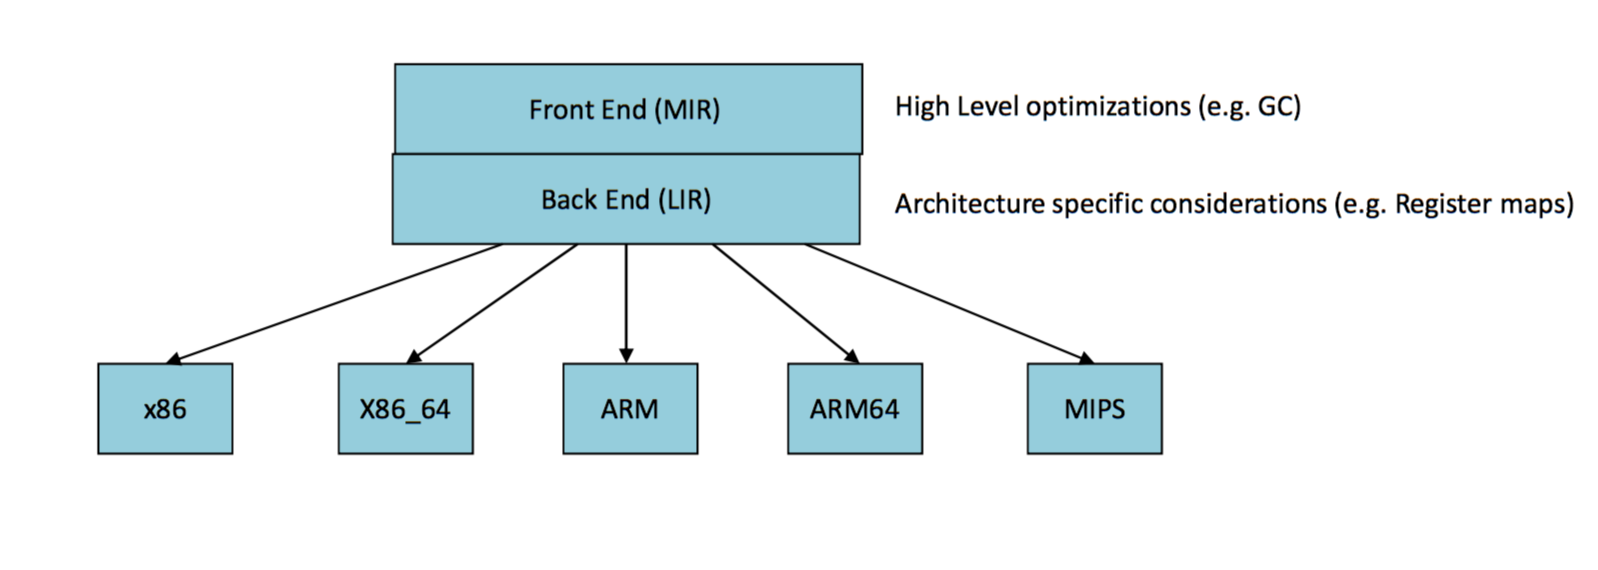
\includegraphics[width=0.8\textwidth]{data/artarch.png}
    \caption{artarch}
    \label{fig:artarch}
\end{figure}
